\documentclass[10pt]{article}
\usepackage[letterpaper,left=0.6in,right=0.6in,top=1.36in,bottom=0.65in,
  footskip=0.3in]{geometry}
\usepackage[T1]{fontenc}
\usepackage{tgheros}
\renewcommand{\familydefault}{\sfdefault}
\usepackage[final,stretch=12,shrink=12]{microtype}
\usepackage{xcolor}
\definecolor{ckteal}{HTML}{3F8F80}
\definecolor{ckpale}{HTML}{EAF4F1}
\definecolor{ckink}{HTML}{1E2A2E}
\definecolor{ckmuted}{HTML}{66737A}
\usepackage{graphicx}
\usepackage{multicol}
\usepackage{tikz}
\usepackage[most]{tcolorbox}
\usepackage{fancyhdr}
\usepackage{titlesec}
\usepackage{enumitem}
\usepackage{hyperref}
\hypersetup{colorlinks=true,urlcolor=ckteal,linkcolor=ckteal,
  pdftitle={Calkit: Continuously integrated{,} transparent{,} reproducible science in the age of agentic AI},pdfauthor={Calkit}}
% What pandoc's LaTeX writer leans on
\providecommand{\tightlist}{%
  \setlength{\itemsep}{0pt}\setlength{\parskip}{0pt}}
\providecommand{\pandocbounded}[1]{#1}
% A value from a results file; calkit.sty defines this to record where it
% came from, and without it a value prints as itself
\providecommand{\ckvalue}[4]{#2}
% One headline number and what it measures
\newcommand{\cknumber}[2]{%
  \par\noindent
  \begin{minipage}[c]{0.36\linewidth}\raggedleft
    {\color{ckteal}\fontsize{23}{25}\selectfont\bfseries #1}%
  \end{minipage}\hfill
  \begin{minipage}[c]{0.6\linewidth}\raggedright
    \small\color{ckink}#2%
  \end{minipage}\par\vspace{5pt}}
\color{ckink}
\setlength{\parindent}{0pt}
\setlength{\parskip}{5pt}
\setlength{\columnsep}{0.3in}
\setlist{leftmargin=1.2em,itemsep=1pt,topsep=2pt}
\titleformat{\section}{\color{ckteal}\bfseries\large}{}{0pt}{}
\titlespacing*{\section}{0pt}{8pt}{2pt}
\pagestyle{fancy}
\fancyhf{}
\renewcommand{\headrulewidth}{0pt}
\fancyfoot[C]{\color{ckmuted}\scriptsize Built by Calkit v0.48.1.dev40 from \href{https://calkit.io/calkit/calkit?ref=bca499ddded49ec46eef63d16fc187eea5e9ead4}{calkit.io/calkit/calkit} at rev \texttt{bca499d}.}
% It's a one-pager, so spilling onto a second page is an error, not a
% layout to live with
\AtEndDocument{\ifnum\value{page}>1
  \GenericError{}{The one-pager runs to \arabic{page} pages}{}{}\fi}
\begin{document}
\begin{tikzpicture}[remember picture,overlay]
  \fill[ckteal] (current page.north west)
    rectangle ([yshift=-1.18in]current page.north east);
  \node[anchor=west,text width=7.3in,align=left,text=white,
    font=\bfseries\fontsize{18}{22}\selectfont]
    at ([xshift=0.6in,yshift=-0.6in]current page.north west) {\emph{Calkit}:
Continuously integrated, transparent, reproducible science in the age of
agentic AI};
\end{tikzpicture}
\noindent
\begin{minipage}[c]{0.6\linewidth}
  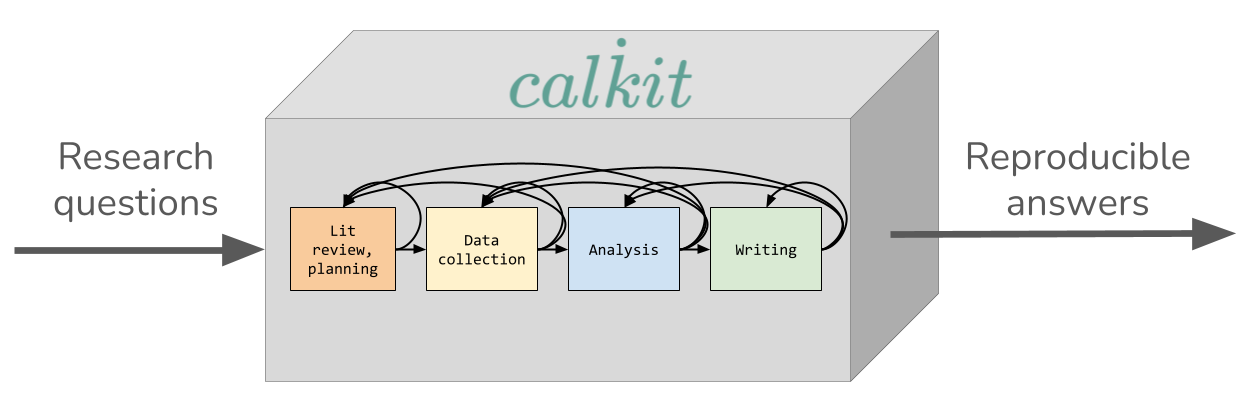
\includegraphics[width=\linewidth]{../img/pipeline.png}
\end{minipage}\hfill
\begin{minipage}[c]{0.37\linewidth}
  \begin{tcolorbox}[colback=ckpale,colframe=ckpale,boxrule=0pt,arc=4pt,
    left=8pt,right=8pt,top=6pt,bottom=4pt]
    {\color{ckteal}\bfseries\small BY THE NUMBERS}\par\vspace{4pt}
    \cknumber{\href{https://calkit.io/calkit/calkit/questions/1?ref=bca499ddded49ec46eef63d16fc187eea5e9ead4}{\ckvalue{goals.steps.1.student\_days\_gain}{24\%}{results/research-flow.json}{research-flow}}}{more papers in a PhD with agents alone}
    \cknumber{\href{https://calkit.io/calkit/calkit/questions/1?ref=bca499ddded49ec46eef63d16fc187eea5e9ead4}{\ckvalue{goals.student\_days\_gain}{99\%}{results/research-flow.json}{research-flow}}}{more with agents and Calkit}
        {\scriptsize\color{ckmuted}Simulated in
\href{https://calkit.io/calkit/calkit/pipeline?stage=research-flow&ref=bca499ddded49ec46eef63d16fc187eea5e9ead4}{Calkit's
own pipeline}.}
      \end{tcolorbox}
\end{minipage}
\par\vspace{6pt}
\begin{multicols}{2}
\fontsize{10.6}{14}\selectfont
% Justified, breaking words only now and then, and never names, e.g.,
% MATLAB
\uchyph=0\hyphenpenalty=500\tolerance=1000\emergencystretch=0.8em
Generative AI is making it much cheaper to produce research outputs,
while the reproducibility crisis remains unsolved
(\href{https://doi.org/10.1371/journal.pone.0311493}{only 12\% of
studies share code}, and even fewer share code that is quick to verify).
As the bottleneck is shifting from producing outputs to checking that
those outputs are trustworthy, it's now more important than ever to make
it intuitive and enjoyable to work transparently and reproducibly, both
for humans and AI agents.

Rather than assuming we should simply teach scientists software
development tools and platforms and leave them to assemble their own
workflows (the status quo, which seems to have saturated), Calkit
provides a vertically-integrated, research-focused experience right out
of the box: reference management, version control (including large data
files), computational environments, pipeline automation, and a
web-based, self-hostable collaboration platform.

Calkit is designed to help individuals work more efficiently by allowing
all stages of research---from asking questions, to data collection and
analysis, to publication---to live together in the same project,
breaking down silos that slow down iteration while allowing more
inclusive collaboration, i.e., from those who don't want to or need to
learn complex tools like Git. A Calkit project includes the research
article, not only supplements it, and is intended to be shipped whole,
providing full context and lighting fast verifiability, by linking all
evidence for answers to research questions back to reproducible
calculations.

\section{A success story}\label{a-success-story}

Rebecca McCabe recently finished her PhD in Mechanical Engineering at
Cornell. She used Calkit to create a single-button reproducible pipeline
that integrated MATLAB, Python, Julia, LaTeX, and more. She used
Calkit's Overleaf integration to allow collaborators to contribute
without learning Git.

\section{Where we're heading and what support we
need}\label{where-were-heading-and-what-support-we-need}

Calkit is developed and operated in a very lean and efficient manner.
We're currently supported with 25\% of a Sr.~Research Software
Engineer's capacity provided by the Schmidt Academy for Software
Engineering at Caltech. Google Cloud has generously provided credits to
run the cloud infrastructure for a year, and we need \$5k to stay
running for another.

With an MVP in place serving a handful of users, we now need to do some
training and community building by hosting workshops, starting around
Southern California and Boston. These will be focused on computational
reproducibility principles, with Calkit positioned as one, not the only
way to achieve them. Through these efforts we're looking to 10x our user
base and continue to evolve the software to increase the number of
comprehensive, transparent, single-button reproducible research projects
released alongside papers. To do this, we're seeking \$75k for 2027.

\section{Learn more}\label{learn-more}

To learn more about Calkit, you can check out
\href{http://docs.calkit.org}{the docs} and try out the web platform at
\href{http://calkit.io}{calkit.io}.
\end{multicols}
\end{document}
